\worksheet{Tiger's Consistency}

To model a round of golf, roll two dice You score 70 with a roll that sums to 7. A sum of 6 corresponds to scoring one stroke below 70 (69), and a sum of 8, one stroke above (71). Foe each number below a sum of 6, we'll subtract two additional strokes, and for each number above a sum of 8, we'll add two strokes.
\begin{enumerate}
	\item Is it possible to score a 74 using this simulation? Why or why not? \vfill
	\item Fill in the table for the dice roll model:
	
	\begin{center} \Large
		\begin{tabular}{c|c}
		Dice Roll & Round Score\\\hline
		4 & \\\hline
		5 & \\\hline
		6 & 69\\\hline
		7 & 70\\\hline
		8 & 71\\\hline
		9 & \\\hline
		10 & \\\hline
		\end{tabular}
	\end{center}\normalsize
	
	\item How well does the model fit the statement ``In the PGA, the average first round score is about 70 with a standard deviation of about 4.''
	\begin{enumerate}
		\item What scores would be included in the statement ``within one standard deviation of the mean''?\vfill
		\item What percentage of the rounds should be within one standard deviation of the mean? \label{tiger1}\vfill
		\item How many different dice rolls will give you scores within one standard deviation of the mean? \label{tiger2}
		\begin{center} \large
			\begin{tabular}{c*{6}{|c}}
			 & 1 & 2 & 3 & 4 & 5 & 6\\\hline
			1&&&&&&\\\hline
			2&&&&&&\\\hline
			3&&&&&&\\\hline
			4&&&&&&\\\hline
			5&&&&&&\\\hline
			6&&&&&&\\\hline
			\end{tabular}
		\end{center}\normalsize
		\item Do your answers to question \ref{tiger1} and \ref{tiger2} agree?
	\end{enumerate}
	
	\clearpage
	\item We will say that the cut for the first two rounds of a tournament is 140. Can you make the cut in thirty straight tournaments?
	\begin{enumerate}
		\item Roll four dice (or a single die four times or a pair of dice twice) and calculate the sum.
		\item Score two die at a time. If your total score is 140 or less, you make the cut. Mark a box in the grid below.
		\item if the sum is over 140 you do not make the cut, and your streak ends.
		\begin{center} \Large
			\begin{tabular}{c*{5}{|p{1cm}}}\hline
			Round 1 score & & & & &\\\hline
			Round 2 score & & & & &\\\hline
			Make the cut (\(X\)) & & & & &\\\hline
			\end{tabular}\normalsize
			
	\end{center}
	\item The book says not to bother calculating your score for each round individually, but just deciding that you make the cut if your four dice sum up to 14 or less. Is it possible for you to make the cut and have your dice add up to something larger than 14? Is it possible for you to not make the cut and have your dice add up to 14 or smaller?
			
			If you have made the first 5 cuts, continue documenting your streak below based on your calculations.
	\begin{center}
		
		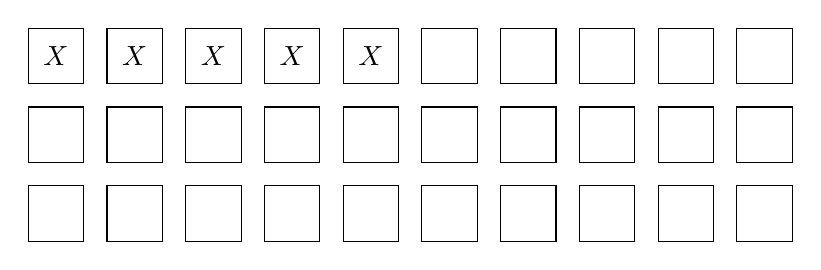
\begin{tikzpicture}
	%\node at (0,0) {$\checkmark$};
		 \foreach \x in {1,...,10}{
		\foreach \y in {0,...,2}{
       \node [inner sep=10pt, draw] at  (\x,\y)  {};
       }
			}
		\foreach \x in {1,..., 5}{
		\node [] at  (\x,2)  {\(X\)};
		}
	\end{tikzpicture}
		\end{center}
		
		\item Type ``number of ways to roll 4 dice with a sum \(<=\) 14 into \texttt{WolframAlpha.com}. Use this to calculate the probability of making the cut in 30 tournaments in a row. \label{tiger3}
		
	\end{enumerate}
		\item Based on Tiger Wood's golfing ability, the book shows that Tiger Woods gains, on average, more than two strokes per round. This is then used to decide that Tiger makes the cut when the four dice roll sums to 16 or less. Explain the reasoning behind this change. \vfill
		\item Based on Tiger Wood's consist play, the book reduces his standard deviation from 4 holes per round to 2 holes per round. They do this by assigning him a 68 for a two-dice sum of 7 and only adding one stroke for each number above and below 7.  Fill in the table again.
		
		\begin{center} \Large
		\begin{tabular}{c|c}
		Dice Roll & Round Score\\\hline
		4 & \\\hline
		5 & \\\hline
		6 & \\\hline
		7 & 68\\\hline
		8 & \\\hline
		9 & \\\hline
		10 & \\\hline
		\end{tabular}
	\end{center}\normalsize
\item If you take a four-dice roll of 18 or less to make the cut, what is Wood's probability of making the cut in 1 tournament? Explain using your work above why this dice cut-off for the cut based on your work above.
%You may want to use \texttt{WolframAlpha.com} again. What is the probability that he makes the cut in 30 tournaments in a row? Compare that with your answer to \ref{tiger3}. \vfill
\end{enumerate}